\chapter{Background}
When designing the new Autograder front-end, it was necessary to develop other parts of the system for emulating dummy data for the project. One of the most conventional ways of doing this is to create a database that stores the dummy data, and have a server serve the front-end with that data. The system works in many ways as the fully functional Autograder, with methods for communications so that the new front-end can be implemented and deployed with a relatively small amount of effort. Making these methods require us to both think about the current needs and future needs. It is however, no small task to create these sub-systems. We will go though some of the technologies we are using in this chapter.

\section{Front-end}
One of the goals of the new Autograder front-end are to create a better and faster experience for the end-user. This means reflecting on the old design and expierence, and revisit the technologies and code written in the old Autograder front-end. This section describes the libraries and frameworks used for the new front-end.

\subsection{HTML, CSS and Bootstrap}
Hyper text markup language, or HTML, is a markup language used to build websites. Content is placed inside of different Document Object Models, or DOM-elements. The different boxes of content is styled using a cascading style sheet, or CSS. Making the websites and layouts can take a lot of time. To simplify this, there are many open source project that supply off-the-shelf elements. Since we have experience with Bootstrap from earlier projects, it was decided that we would use Bootstrap 3.0 \cite{bootstrap} for the new front-end. The framework is in it's third iteration (soon 4th with Bootstrap 4.0 Alpha being shipped early 2016). The framework comes with build in styling, so the job of the designer (or rather lack of designers) is made easier. Compared to vanilla coding in HTML and CSS, the framework can remove countless hours of coding, and the results look clean and functional. The website is made responsive through a column-system that can change based on the client's screensize. The site becomes more mobile-friendy out of the box, however, it is not a fully optimized. The code must be tweaked to make the site optimized for all devices. With Autograder, column layout is used on all pages.

\subsection{ReactJS}
JavaScript is used to manipulate content on a website. Binding a data model to the DOM is necessary to have an always up-to-date website. Handlers for buttons and inputs are also handled in JavaScript. Handling all event listeners and functions connected to the DOM can be hard, especially when the application is as big as Autograder. Since the front-end communicates with a server, data will come in asynchronously and must trigger a re-render of the DOM-elements. This process of updating and binding data can be implemented using libraries such as ReactJS. React is an open source JavaScript library designed and maintained by Facebook \cite{facebookreact} . The library provides a view for data rendered as HTML, and maintains a state that can change depending on the data that comes from the server. If the data in the server changes, the change are reflected on the page in real-time. Say for example that the users permissions are changed from Student to Teacher. The front-end will have to reflect that change, and show data relevant for a teacher. With React, this change can be made without having to refresh the page manually. 

The choice between ReactJS and AngularJS (the other major JavaScript-library in the industry) is really based on preference. The component based pipeline that React offers is very appealing when the website will recycle a lot of the same elements. The new front-end can be compared to a single-page-application, where the different pages are loaded in without refreshing the page. Navigating between pages will therefore be very fast since the page will not be reloaded. Consequently, a lot of elements must be loaded and unloaded. React uses Virtual DOM to run its Tree Diff algorithm \cite{reacttreediff} and figures out what parts of the DOM should be rendered, this enables quick re-rendering of only relevant for the change components. Components also hold methods such as \emph{componentWillMount()} and \emph{componentShouldMount()} to enable a greater control of data and elements being rendered on the page.

\begin{figure}[h]
\centering
\scalebox{0.5}{{% Graphic for TeX using PGF
% Title: /home/tomgli/workspace/github.com/bachopp/thesis/files/chapters/background/graphs/reactdiffdiagramthin.dia
% Creator: Dia v0.97.3
% CreationDate: Sat Apr 23 13:55:59 2016
% For: tomgli
% \usepackage{tikz}
% The following commands are not supported in PSTricks at present
% We define them conditionally, so when they are implemented,
% this pgf file will use them.
\ifx\du\undefined
  \newlength{\du}
\fi
\setlength{\du}{15\unitlength}
\begin{tikzpicture}
\pgftransformxscale{1.000000}
\pgftransformyscale{-1.000000}
\definecolor{dialinecolor}{rgb}{0.000000, 0.000000, 0.000000}
\pgfsetstrokecolor{dialinecolor}
\definecolor{dialinecolor}{rgb}{1.000000, 1.000000, 1.000000}
\pgfsetfillcolor{dialinecolor}
\definecolor{dialinecolor}{rgb}{1.000000, 1.000000, 1.000000}
\pgfsetfillcolor{dialinecolor}
\pgfpathellipse{\pgfpoint{34.909398\du}{57.597439\du}}{\pgfpoint{0.922067\du}{0\du}}{\pgfpoint{0\du}{0.874328\du}}
\pgfusepath{fill}
\pgfsetlinewidth{0.100000\du}
\pgfsetdash{}{0pt}
\pgfsetdash{}{0pt}
\pgfsetmiterjoin
\definecolor{dialinecolor}{rgb}{0.000000, 0.000000, 0.000000}
\pgfsetstrokecolor{dialinecolor}
\pgfpathellipse{\pgfpoint{34.909398\du}{57.597439\du}}{\pgfpoint{0.922067\du}{0\du}}{\pgfpoint{0\du}{0.874328\du}}
\pgfusepath{stroke}
% setfont left to latex
\definecolor{dialinecolor}{rgb}{0.000000, 0.000000, 0.000000}
\pgfsetstrokecolor{dialinecolor}
\node at (34.909398\du,57.792439\du){};
\definecolor{dialinecolor}{rgb}{1.000000, 1.000000, 1.000000}
\pgfsetfillcolor{dialinecolor}
\pgfpathellipse{\pgfpoint{34.925608\du}{60.858968\du}}{\pgfpoint{0.922067\du}{0\du}}{\pgfpoint{0\du}{0.874328\du}}
\pgfusepath{fill}
\pgfsetlinewidth{0.100000\du}
\pgfsetdash{}{0pt}
\pgfsetdash{}{0pt}
\pgfsetmiterjoin
\definecolor{dialinecolor}{rgb}{0.000000, 0.000000, 0.000000}
\pgfsetstrokecolor{dialinecolor}
\pgfpathellipse{\pgfpoint{34.925608\du}{60.858968\du}}{\pgfpoint{0.922067\du}{0\du}}{\pgfpoint{0\du}{0.874328\du}}
\pgfusepath{stroke}
% setfont left to latex
\definecolor{dialinecolor}{rgb}{0.000000, 0.000000, 0.000000}
\pgfsetstrokecolor{dialinecolor}
\node at (34.925608\du,61.053968\du){};
\definecolor{dialinecolor}{rgb}{1.000000, 1.000000, 1.000000}
\pgfsetfillcolor{dialinecolor}
\pgfpathellipse{\pgfpoint{39.675251\du}{57.895710\du}}{\pgfpoint{0.922067\du}{0\du}}{\pgfpoint{0\du}{0.874328\du}}
\pgfusepath{fill}
\pgfsetlinewidth{0.100000\du}
\pgfsetdash{}{0pt}
\pgfsetdash{}{0pt}
\pgfsetmiterjoin
\definecolor{dialinecolor}{rgb}{0.000000, 0.000000, 0.000000}
\pgfsetstrokecolor{dialinecolor}
\pgfpathellipse{\pgfpoint{39.675251\du}{57.895710\du}}{\pgfpoint{0.922067\du}{0\du}}{\pgfpoint{0\du}{0.874328\du}}
\pgfusepath{stroke}
% setfont left to latex
\definecolor{dialinecolor}{rgb}{0.000000, 0.000000, 0.000000}
\pgfsetstrokecolor{dialinecolor}
\node at (39.675251\du,58.090710\du){};
\definecolor{dialinecolor}{rgb}{1.000000, 0.509804, 0.509804}
\pgfsetfillcolor{dialinecolor}
\pgfpathellipse{\pgfpoint{38.686418\du}{62.486491\du}}{\pgfpoint{0.922067\du}{0\du}}{\pgfpoint{0\du}{0.874328\du}}
\pgfusepath{fill}
\pgfsetlinewidth{0.100000\du}
\pgfsetdash{}{0pt}
\pgfsetdash{}{0pt}
\pgfsetmiterjoin
\definecolor{dialinecolor}{rgb}{0.000000, 0.000000, 0.000000}
\pgfsetstrokecolor{dialinecolor}
\pgfpathellipse{\pgfpoint{38.686418\du}{62.486491\du}}{\pgfpoint{0.922067\du}{0\du}}{\pgfpoint{0\du}{0.874328\du}}
\pgfusepath{stroke}
% setfont left to latex
\definecolor{dialinecolor}{rgb}{0.000000, 0.000000, 0.000000}
\pgfsetstrokecolor{dialinecolor}
\node at (38.686418\du,62.681491\du){};
\definecolor{dialinecolor}{rgb}{0.898039, 0.898039, 0.898039}
\pgfsetfillcolor{dialinecolor}
\fill (48.025035\du,46.743799\du)--(48.025035\du,48.643799\du)--(51.299533\du,48.643799\du)--(51.299533\du,46.743799\du)--cycle;
\pgfsetlinewidth{0.100000\du}
\pgfsetdash{}{0pt}
\pgfsetdash{}{0pt}
\pgfsetmiterjoin
\definecolor{dialinecolor}{rgb}{0.549020, 0.549020, 0.549020}
\pgfsetstrokecolor{dialinecolor}
\draw (48.025035\du,46.743799\du)--(48.025035\du,48.643799\du)--(51.299533\du,48.643799\du)--(51.299533\du,46.743799\du)--cycle;
% setfont left to latex
\definecolor{dialinecolor}{rgb}{0.000000, 0.000000, 0.000000}
\pgfsetstrokecolor{dialinecolor}
\node at (49.662284\du,47.888799\du){};
\definecolor{dialinecolor}{rgb}{0.898039, 0.898039, 0.898039}
\pgfsetfillcolor{dialinecolor}
\fill (46.210841\du,49.629967\du)--(46.210841\du,51.529967\du)--(49.485338\du,51.529967\du)--(49.485338\du,49.629967\du)--cycle;
\pgfsetlinewidth{0.100000\du}
\pgfsetdash{}{0pt}
\pgfsetdash{}{0pt}
\pgfsetmiterjoin
\definecolor{dialinecolor}{rgb}{0.549020, 0.549020, 0.549020}
\pgfsetstrokecolor{dialinecolor}
\draw (46.210841\du,49.629967\du)--(46.210841\du,51.529967\du)--(49.485338\du,51.529967\du)--(49.485338\du,49.629967\du)--cycle;
% setfont left to latex
\definecolor{dialinecolor}{rgb}{0.000000, 0.000000, 0.000000}
\pgfsetstrokecolor{dialinecolor}
\node at (47.848090\du,50.774967\du){};
\definecolor{dialinecolor}{rgb}{0.898039, 0.898039, 0.898039}
\pgfsetfillcolor{dialinecolor}
\fill (50.571434\du,49.649420\du)--(50.571434\du,51.549420\du)--(53.845932\du,51.549420\du)--(53.845932\du,49.649420\du)--cycle;
\pgfsetlinewidth{0.100000\du}
\pgfsetdash{}{0pt}
\pgfsetdash{}{0pt}
\pgfsetmiterjoin
\definecolor{dialinecolor}{rgb}{0.549020, 0.549020, 0.549020}
\pgfsetstrokecolor{dialinecolor}
\draw (50.571434\du,49.649420\du)--(50.571434\du,51.549420\du)--(53.845932\du,51.549420\du)--(53.845932\du,49.649420\du)--cycle;
% setfont left to latex
\definecolor{dialinecolor}{rgb}{0.000000, 0.000000, 0.000000}
\pgfsetstrokecolor{dialinecolor}
\node at (52.208683\du,50.794420\du){};
\definecolor{dialinecolor}{rgb}{0.898039, 0.898039, 0.898039}
\pgfsetfillcolor{dialinecolor}
\fill (44.038649\du,52.385733\du)--(44.038649\du,54.285733\du)--(47.313147\du,54.285733\du)--(47.313147\du,52.385733\du)--cycle;
\pgfsetlinewidth{0.100000\du}
\pgfsetdash{}{0pt}
\pgfsetdash{}{0pt}
\pgfsetmiterjoin
\definecolor{dialinecolor}{rgb}{0.549020, 0.549020, 0.549020}
\pgfsetstrokecolor{dialinecolor}
\draw (44.038649\du,52.385733\du)--(44.038649\du,54.285733\du)--(47.313147\du,54.285733\du)--(47.313147\du,52.385733\du)--cycle;
% setfont left to latex
\definecolor{dialinecolor}{rgb}{0.000000, 0.000000, 0.000000}
\pgfsetstrokecolor{dialinecolor}
\node at (45.675898\du,53.530733\du){};
\definecolor{dialinecolor}{rgb}{0.898039, 0.898039, 0.898039}
\pgfsetfillcolor{dialinecolor}
\fill (48.399243\du,52.405185\du)--(48.399243\du,54.305185\du)--(51.673740\du,54.305185\du)--(51.673740\du,52.405185\du)--cycle;
\pgfsetlinewidth{0.100000\du}
\pgfsetdash{}{0pt}
\pgfsetdash{}{0pt}
\pgfsetmiterjoin
\definecolor{dialinecolor}{rgb}{0.549020, 0.549020, 0.549020}
\pgfsetstrokecolor{dialinecolor}
\draw (48.399243\du,52.405185\du)--(48.399243\du,54.305185\du)--(51.673740\du,54.305185\du)--(51.673740\du,52.405185\du)--cycle;
% setfont left to latex
\definecolor{dialinecolor}{rgb}{0.000000, 0.000000, 0.000000}
\pgfsetstrokecolor{dialinecolor}
\node at (50.036492\du,53.550185\du){};
\definecolor{dialinecolor}{rgb}{0.898039, 0.898039, 0.898039}
\pgfsetfillcolor{dialinecolor}
\fill (48.512715\du,55.368444\du)--(48.512715\du,57.268444\du)--(51.787213\du,57.268444\du)--(51.787213\du,55.368444\du)--cycle;
\pgfsetlinewidth{0.100000\du}
\pgfsetdash{}{0pt}
\pgfsetdash{}{0pt}
\pgfsetmiterjoin
\definecolor{dialinecolor}{rgb}{0.549020, 0.549020, 0.549020}
\pgfsetstrokecolor{dialinecolor}
\draw (48.512715\du,55.368444\du)--(48.512715\du,57.268444\du)--(51.787213\du,57.268444\du)--(51.787213\du,55.368444\du)--cycle;
% setfont left to latex
\definecolor{dialinecolor}{rgb}{0.000000, 0.000000, 0.000000}
\pgfsetstrokecolor{dialinecolor}
\node at (50.149964\du,56.513444\du){};
\definecolor{dialinecolor}{rgb}{1.000000, 1.000000, 1.000000}
\pgfsetfillcolor{dialinecolor}
\pgfpathellipse{\pgfpoint{31.922753\du}{56.062026\du}}{\pgfpoint{0.922067\du}{0\du}}{\pgfpoint{0\du}{0.874328\du}}
\pgfusepath{fill}
\pgfsetlinewidth{0.100000\du}
\pgfsetdash{}{0pt}
\pgfsetdash{}{0pt}
\pgfsetmiterjoin
\definecolor{dialinecolor}{rgb}{0.000000, 0.000000, 0.000000}
\pgfsetstrokecolor{dialinecolor}
\pgfpathellipse{\pgfpoint{31.922753\du}{56.062026\du}}{\pgfpoint{0.922067\du}{0\du}}{\pgfpoint{0\du}{0.874328\du}}
\pgfusepath{stroke}
% setfont left to latex
\definecolor{dialinecolor}{rgb}{0.000000, 0.000000, 0.000000}
\pgfsetstrokecolor{dialinecolor}
\node at (31.922753\du,56.257026\du){};
\definecolor{dialinecolor}{rgb}{0.898039, 0.898039, 0.898039}
\pgfsetfillcolor{dialinecolor}
\fill (47.984149\du,61.262534\du)--(47.984149\du,63.162534\du)--(51.258647\du,63.162534\du)--(51.258647\du,61.262534\du)--cycle;
\pgfsetlinewidth{0.100000\du}
\pgfsetdash{}{0pt}
\pgfsetdash{}{0pt}
\pgfsetmiterjoin
\definecolor{dialinecolor}{rgb}{0.549020, 0.549020, 0.549020}
\pgfsetstrokecolor{dialinecolor}
\draw (47.984149\du,61.262534\du)--(47.984149\du,63.162534\du)--(51.258647\du,63.162534\du)--(51.258647\du,61.262534\du)--cycle;
% setfont left to latex
\definecolor{dialinecolor}{rgb}{0.000000, 0.000000, 0.000000}
\pgfsetstrokecolor{dialinecolor}
\node at (49.621398\du,62.407534\du){};
\definecolor{dialinecolor}{rgb}{0.898039, 0.898039, 0.898039}
\pgfsetfillcolor{dialinecolor}
\fill (46.169955\du,64.148703\du)--(46.169955\du,66.048703\du)--(49.444453\du,66.048703\du)--(49.444453\du,64.148703\du)--cycle;
\pgfsetlinewidth{0.100000\du}
\pgfsetdash{}{0pt}
\pgfsetdash{}{0pt}
\pgfsetmiterjoin
\definecolor{dialinecolor}{rgb}{0.549020, 0.549020, 0.549020}
\pgfsetstrokecolor{dialinecolor}
\draw (46.169955\du,64.148703\du)--(46.169955\du,66.048703\du)--(49.444453\du,66.048703\du)--(49.444453\du,64.148703\du)--cycle;
% setfont left to latex
\definecolor{dialinecolor}{rgb}{0.000000, 0.000000, 0.000000}
\pgfsetstrokecolor{dialinecolor}
\node at (47.807204\du,65.293703\du){};
\definecolor{dialinecolor}{rgb}{0.898039, 0.898039, 0.898039}
\pgfsetfillcolor{dialinecolor}
\fill (50.530549\du,64.168155\du)--(50.530549\du,66.068155\du)--(53.805046\du,66.068155\du)--(53.805046\du,64.168155\du)--cycle;
\pgfsetlinewidth{0.100000\du}
\pgfsetdash{}{0pt}
\pgfsetdash{}{0pt}
\pgfsetmiterjoin
\definecolor{dialinecolor}{rgb}{0.549020, 0.549020, 0.549020}
\pgfsetstrokecolor{dialinecolor}
\draw (50.530549\du,64.168155\du)--(50.530549\du,66.068155\du)--(53.805046\du,66.068155\du)--(53.805046\du,64.168155\du)--cycle;
% setfont left to latex
\definecolor{dialinecolor}{rgb}{0.000000, 0.000000, 0.000000}
\pgfsetstrokecolor{dialinecolor}
\node at (52.167798\du,65.313155\du){};
\definecolor{dialinecolor}{rgb}{1.000000, 0.509804, 0.509804}
\pgfsetfillcolor{dialinecolor}
\fill (43.997764\du,66.904468\du)--(43.997764\du,68.804468\du)--(47.272261\du,68.804468\du)--(47.272261\du,66.904468\du)--cycle;
\pgfsetlinewidth{0.100000\du}
\pgfsetdash{}{0pt}
\pgfsetdash{}{0pt}
\pgfsetmiterjoin
\definecolor{dialinecolor}{rgb}{0.549020, 0.549020, 0.549020}
\pgfsetstrokecolor{dialinecolor}
\draw (43.997764\du,66.904468\du)--(43.997764\du,68.804468\du)--(47.272261\du,68.804468\du)--(47.272261\du,66.904468\du)--cycle;
% setfont left to latex
\definecolor{dialinecolor}{rgb}{0.000000, 0.000000, 0.000000}
\pgfsetstrokecolor{dialinecolor}
\node at (45.635013\du,68.049468\du){};
\definecolor{dialinecolor}{rgb}{0.898039, 0.898039, 0.898039}
\pgfsetfillcolor{dialinecolor}
\fill (48.358357\du,66.923920\du)--(48.358357\du,68.823920\du)--(51.632855\du,68.823920\du)--(51.632855\du,66.923920\du)--cycle;
\pgfsetlinewidth{0.100000\du}
\pgfsetdash{}{0pt}
\pgfsetdash{}{0pt}
\pgfsetmiterjoin
\definecolor{dialinecolor}{rgb}{0.549020, 0.549020, 0.549020}
\pgfsetstrokecolor{dialinecolor}
\draw (48.358357\du,66.923920\du)--(48.358357\du,68.823920\du)--(51.632855\du,68.823920\du)--(51.632855\du,66.923920\du)--cycle;
% setfont left to latex
\definecolor{dialinecolor}{rgb}{0.000000, 0.000000, 0.000000}
\pgfsetstrokecolor{dialinecolor}
\node at (49.995606\du,68.068920\du){};
\definecolor{dialinecolor}{rgb}{0.898039, 0.898039, 0.898039}
\pgfsetfillcolor{dialinecolor}
\fill (48.471830\du,69.887179\du)--(48.471830\du,71.787179\du)--(51.746328\du,71.787179\du)--(51.746328\du,69.887179\du)--cycle;
\pgfsetlinewidth{0.100000\du}
\pgfsetdash{}{0pt}
\pgfsetdash{}{0pt}
\pgfsetmiterjoin
\definecolor{dialinecolor}{rgb}{0.549020, 0.549020, 0.549020}
\pgfsetstrokecolor{dialinecolor}
\draw (48.471830\du,69.887179\du)--(48.471830\du,71.787179\du)--(51.746328\du,71.787179\du)--(51.746328\du,69.887179\du)--cycle;
% setfont left to latex
\definecolor{dialinecolor}{rgb}{0.000000, 0.000000, 0.000000}
\pgfsetstrokecolor{dialinecolor}
\node at (50.109079\du,71.032179\du){};
\definecolor{dialinecolor}{rgb}{1.000000, 1.000000, 1.000000}
\pgfsetfillcolor{dialinecolor}
\fill (67.651782\du,54.752294\du)--(67.651782\du,56.652294\du)--(70.926279\du,56.652294\du)--(70.926279\du,54.752294\du)--cycle;
\pgfsetlinewidth{0.100000\du}
\pgfsetdash{}{0pt}
\pgfsetdash{}{0pt}
\pgfsetmiterjoin
\definecolor{dialinecolor}{rgb}{0.000000, 0.000000, 0.000000}
\pgfsetstrokecolor{dialinecolor}
\draw (67.651782\du,54.752294\du)--(67.651782\du,56.652294\du)--(70.926279\du,56.652294\du)--(70.926279\du,54.752294\du)--cycle;
% setfont left to latex
\definecolor{dialinecolor}{rgb}{0.000000, 0.000000, 0.000000}
\pgfsetstrokecolor{dialinecolor}
\node at (69.289030\du,55.897294\du){};
\definecolor{dialinecolor}{rgb}{1.000000, 1.000000, 1.000000}
\pgfsetfillcolor{dialinecolor}
\fill (65.837587\du,57.638463\du)--(65.837587\du,59.538463\du)--(69.112085\du,59.538463\du)--(69.112085\du,57.638463\du)--cycle;
\pgfsetlinewidth{0.100000\du}
\pgfsetdash{}{0pt}
\pgfsetdash{}{0pt}
\pgfsetmiterjoin
\definecolor{dialinecolor}{rgb}{0.000000, 0.000000, 0.000000}
\pgfsetstrokecolor{dialinecolor}
\draw (65.837587\du,57.638463\du)--(65.837587\du,59.538463\du)--(69.112085\du,59.538463\du)--(69.112085\du,57.638463\du)--cycle;
% setfont left to latex
\definecolor{dialinecolor}{rgb}{0.000000, 0.000000, 0.000000}
\pgfsetstrokecolor{dialinecolor}
\node at (67.474836\du,58.783463\du){};
\definecolor{dialinecolor}{rgb}{1.000000, 1.000000, 1.000000}
\pgfsetfillcolor{dialinecolor}
\fill (70.198181\du,57.657915\du)--(70.198181\du,59.557915\du)--(73.472679\du,59.557915\du)--(73.472679\du,57.657915\du)--cycle;
\pgfsetlinewidth{0.100000\du}
\pgfsetdash{}{0pt}
\pgfsetdash{}{0pt}
\pgfsetmiterjoin
\definecolor{dialinecolor}{rgb}{0.000000, 0.000000, 0.000000}
\pgfsetstrokecolor{dialinecolor}
\draw (70.198181\du,57.657915\du)--(70.198181\du,59.557915\du)--(73.472679\du,59.557915\du)--(73.472679\du,57.657915\du)--cycle;
% setfont left to latex
\definecolor{dialinecolor}{rgb}{0.000000, 0.000000, 0.000000}
\pgfsetstrokecolor{dialinecolor}
\node at (71.835430\du,58.802915\du){};
\definecolor{dialinecolor}{rgb}{1.000000, 0.509804, 0.509804}
\pgfsetfillcolor{dialinecolor}
\fill (63.665396\du,60.394228\du)--(63.665396\du,62.294228\du)--(66.939894\du,62.294228\du)--(66.939894\du,60.394228\du)--cycle;
\pgfsetlinewidth{0.100000\du}
\pgfsetdash{}{0pt}
\pgfsetdash{}{0pt}
\pgfsetmiterjoin
\definecolor{dialinecolor}{rgb}{0.000000, 0.000000, 0.000000}
\pgfsetstrokecolor{dialinecolor}
\draw (63.665396\du,60.394228\du)--(63.665396\du,62.294228\du)--(66.939894\du,62.294228\du)--(66.939894\du,60.394228\du)--cycle;
% setfont left to latex
\definecolor{dialinecolor}{rgb}{0.000000, 0.000000, 0.000000}
\pgfsetstrokecolor{dialinecolor}
\node at (65.302645\du,61.539228\du){};
\definecolor{dialinecolor}{rgb}{1.000000, 1.000000, 1.000000}
\pgfsetfillcolor{dialinecolor}
\fill (68.025989\du,60.413680\du)--(68.025989\du,62.313680\du)--(71.300487\du,62.313680\du)--(71.300487\du,60.413680\du)--cycle;
\pgfsetlinewidth{0.100000\du}
\pgfsetdash{}{0pt}
\pgfsetdash{}{0pt}
\pgfsetmiterjoin
\definecolor{dialinecolor}{rgb}{0.000000, 0.000000, 0.000000}
\pgfsetstrokecolor{dialinecolor}
\draw (68.025989\du,60.413680\du)--(68.025989\du,62.313680\du)--(71.300487\du,62.313680\du)--(71.300487\du,60.413680\du)--cycle;
% setfont left to latex
\definecolor{dialinecolor}{rgb}{0.000000, 0.000000, 0.000000}
\pgfsetstrokecolor{dialinecolor}
\node at (69.663238\du,61.558680\du){};
\definecolor{dialinecolor}{rgb}{1.000000, 1.000000, 1.000000}
\pgfsetfillcolor{dialinecolor}
\fill (68.139462\du,63.376939\du)--(68.139462\du,65.276939\du)--(71.413960\du,65.276939\du)--(71.413960\du,63.376939\du)--cycle;
\pgfsetlinewidth{0.100000\du}
\pgfsetdash{}{0pt}
\pgfsetdash{}{0pt}
\pgfsetmiterjoin
\definecolor{dialinecolor}{rgb}{0.000000, 0.000000, 0.000000}
\pgfsetstrokecolor{dialinecolor}
\draw (68.139462\du,63.376939\du)--(68.139462\du,65.276939\du)--(71.413960\du,65.276939\du)--(71.413960\du,63.376939\du)--cycle;
% setfont left to latex
\definecolor{dialinecolor}{rgb}{0.000000, 0.000000, 0.000000}
\pgfsetstrokecolor{dialinecolor}
\node at (69.776711\du,64.521939\du){};
\pgfsetlinewidth{0.100000\du}
\pgfsetdash{}{0pt}
\pgfsetdash{}{0pt}
\pgfsetmiterjoin
\definecolor{dialinecolor}{rgb}{0.549020, 0.549020, 0.549020}
\pgfsetstrokecolor{dialinecolor}
\pgfpathellipse{\pgfpoint{49.127059\du}{51.603158\du}}{\pgfpoint{6.946203\du}{0\du}}{\pgfpoint{0\du}{6.480362\du}}
\pgfusepath{stroke}
% setfont left to latex
\definecolor{dialinecolor}{rgb}{0.000000, 0.000000, 0.000000}
\pgfsetstrokecolor{dialinecolor}
\node at (49.127059\du,51.798158\du){};
\pgfsetlinewidth{0.100000\du}
\pgfsetdash{}{0pt}
\pgfsetdash{}{0pt}
\pgfsetbuttcap
{
\definecolor{dialinecolor}{rgb}{0.549020, 0.549020, 0.549020}
\pgfsetfillcolor{dialinecolor}
% was here!!!
\definecolor{dialinecolor}{rgb}{0.549020, 0.549020, 0.549020}
\pgfsetstrokecolor{dialinecolor}
\draw (49.034225\du,48.692966\du)--(48.476148\du,49.580801\du);
}
\pgfsetlinewidth{0.100000\du}
\pgfsetdash{}{0pt}
\pgfsetdash{}{0pt}
\pgfsetbuttcap
{
\definecolor{dialinecolor}{rgb}{0.549020, 0.549020, 0.549020}
\pgfsetfillcolor{dialinecolor}
% was here!!!
\definecolor{dialinecolor}{rgb}{0.549020, 0.549020, 0.549020}
\pgfsetstrokecolor{dialinecolor}
\draw (50.538230\du,48.693315\du)--(51.332737\du,49.599903\du);
}
\pgfsetlinewidth{0.100000\du}
\pgfsetdash{}{0pt}
\pgfsetdash{}{0pt}
\pgfsetbuttcap
{
\definecolor{dialinecolor}{rgb}{0.549020, 0.549020, 0.549020}
\pgfsetfillcolor{dialinecolor}
% was here!!!
\definecolor{dialinecolor}{rgb}{0.549020, 0.549020, 0.549020}
\pgfsetstrokecolor{dialinecolor}
\draw (47.059769\du,51.580076\du)--(46.464219\du,52.335624\du);
}
\pgfsetlinewidth{0.100000\du}
\pgfsetdash{}{0pt}
\pgfsetdash{}{0pt}
\pgfsetbuttcap
{
\definecolor{dialinecolor}{rgb}{0.549020, 0.549020, 0.549020}
\pgfsetfillcolor{dialinecolor}
% was here!!!
\definecolor{dialinecolor}{rgb}{0.549020, 0.549020, 0.549020}
\pgfsetstrokecolor{dialinecolor}
\draw (48.635615\du,51.578666\du)--(49.248966\du,52.356486\du);
}
\pgfsetlinewidth{0.100000\du}
\pgfsetdash{}{0pt}
\pgfsetdash{}{0pt}
\pgfsetbuttcap
{
\definecolor{dialinecolor}{rgb}{0.549020, 0.549020, 0.549020}
\pgfsetfillcolor{dialinecolor}
% was here!!!
\definecolor{dialinecolor}{rgb}{0.549020, 0.549020, 0.549020}
\pgfsetstrokecolor{dialinecolor}
\draw (50.074791\du,54.355357\du)--(50.111664\du,55.318272\du);
}
\pgfsetlinewidth{0.100000\du}
\pgfsetdash{}{0pt}
\pgfsetdash{}{0pt}
\pgfsetbuttcap
{
\definecolor{dialinecolor}{rgb}{0.549020, 0.549020, 0.549020}
\pgfsetfillcolor{dialinecolor}
% was here!!!
\definecolor{dialinecolor}{rgb}{0.549020, 0.549020, 0.549020}
\pgfsetstrokecolor{dialinecolor}
\draw (48.993340\du,63.211701\du)--(48.435263\du,64.099536\du);
}
\pgfsetlinewidth{0.100000\du}
\pgfsetdash{}{0pt}
\pgfsetdash{}{0pt}
\pgfsetbuttcap
{
\definecolor{dialinecolor}{rgb}{0.549020, 0.549020, 0.549020}
\pgfsetfillcolor{dialinecolor}
% was here!!!
\definecolor{dialinecolor}{rgb}{0.549020, 0.549020, 0.549020}
\pgfsetstrokecolor{dialinecolor}
\draw (50.497345\du,63.212051\du)--(51.291851\du,64.118638\du);
}
\pgfsetlinewidth{0.100000\du}
\pgfsetdash{}{0pt}
\pgfsetdash{}{0pt}
\pgfsetbuttcap
{
\definecolor{dialinecolor}{rgb}{0.549020, 0.549020, 0.549020}
\pgfsetfillcolor{dialinecolor}
% was here!!!
\definecolor{dialinecolor}{rgb}{0.549020, 0.549020, 0.549020}
\pgfsetstrokecolor{dialinecolor}
\draw (47.018883\du,66.098811\du)--(46.423334\du,66.854359\du);
}
\pgfsetlinewidth{0.100000\du}
\pgfsetdash{}{0pt}
\pgfsetdash{}{0pt}
\pgfsetbuttcap
{
\definecolor{dialinecolor}{rgb}{0.549020, 0.549020, 0.549020}
\pgfsetfillcolor{dialinecolor}
% was here!!!
\definecolor{dialinecolor}{rgb}{0.549020, 0.549020, 0.549020}
\pgfsetstrokecolor{dialinecolor}
\draw (48.594730\du,66.097402\du)--(49.208081\du,66.875221\du);
}
\pgfsetlinewidth{0.100000\du}
\pgfsetdash{}{0pt}
\pgfsetdash{}{0pt}
\pgfsetbuttcap
{
\definecolor{dialinecolor}{rgb}{0.549020, 0.549020, 0.549020}
\pgfsetfillcolor{dialinecolor}
% was here!!!
\definecolor{dialinecolor}{rgb}{0.549020, 0.549020, 0.549020}
\pgfsetstrokecolor{dialinecolor}
\draw (50.033906\du,68.874092\du)--(50.070779\du,69.837007\du);
}
\pgfsetlinewidth{0.100000\du}
\pgfsetdash{}{0pt}
\pgfsetdash{}{0pt}
\pgfsetbuttcap
{
\definecolor{dialinecolor}{rgb}{0.000000, 0.000000, 0.000000}
\pgfsetfillcolor{dialinecolor}
% was here!!!
\definecolor{dialinecolor}{rgb}{0.000000, 0.000000, 0.000000}
\pgfsetstrokecolor{dialinecolor}
\draw (68.660972\du,56.701461\du)--(68.102895\du,57.589296\du);
}
\pgfsetlinewidth{0.100000\du}
\pgfsetdash{}{0pt}
\pgfsetdash{}{0pt}
\pgfsetbuttcap
{
\definecolor{dialinecolor}{rgb}{0.000000, 0.000000, 0.000000}
\pgfsetfillcolor{dialinecolor}
% was here!!!
\definecolor{dialinecolor}{rgb}{0.000000, 0.000000, 0.000000}
\pgfsetstrokecolor{dialinecolor}
\draw (70.164977\du,56.701811\du)--(70.959483\du,57.608398\du);
}
\pgfsetlinewidth{0.100000\du}
\pgfsetdash{}{0pt}
\pgfsetdash{}{0pt}
\pgfsetbuttcap
{
\definecolor{dialinecolor}{rgb}{0.000000, 0.000000, 0.000000}
\pgfsetfillcolor{dialinecolor}
% was here!!!
\definecolor{dialinecolor}{rgb}{0.000000, 0.000000, 0.000000}
\pgfsetstrokecolor{dialinecolor}
\draw (66.686515\du,59.588571\du)--(66.090966\du,60.344119\du);
}
\pgfsetlinewidth{0.100000\du}
\pgfsetdash{}{0pt}
\pgfsetdash{}{0pt}
\pgfsetbuttcap
{
\definecolor{dialinecolor}{rgb}{0.000000, 0.000000, 0.000000}
\pgfsetfillcolor{dialinecolor}
% was here!!!
\definecolor{dialinecolor}{rgb}{0.000000, 0.000000, 0.000000}
\pgfsetstrokecolor{dialinecolor}
\draw (68.262362\du,59.587162\du)--(68.875713\du,60.364981\du);
}
\pgfsetlinewidth{0.100000\du}
\pgfsetdash{}{0pt}
\pgfsetdash{}{0pt}
\pgfsetbuttcap
{
\definecolor{dialinecolor}{rgb}{0.000000, 0.000000, 0.000000}
\pgfsetfillcolor{dialinecolor}
% was here!!!
\definecolor{dialinecolor}{rgb}{0.000000, 0.000000, 0.000000}
\pgfsetstrokecolor{dialinecolor}
\draw (69.701538\du,62.363852\du)--(69.738411\du,63.326767\du);
}
\definecolor{dialinecolor}{rgb}{1.000000, 0.509804, 0.509804}
\pgfsetfillcolor{dialinecolor}
\fill (56.489531\du,58.272316\du)--(56.489531\du,60.172316\du)--(59.764029\du,60.172316\du)--(59.764029\du,58.272316\du)--cycle;
\pgfsetlinewidth{0.100000\du}
\pgfsetdash{}{0pt}
\pgfsetdash{}{0pt}
\pgfsetmiterjoin
\definecolor{dialinecolor}{rgb}{0.000000, 0.000000, 0.000000}
\pgfsetstrokecolor{dialinecolor}
\draw (56.489531\du,58.272316\du)--(56.489531\du,60.172316\du)--(59.764029\du,60.172316\du)--(59.764029\du,58.272316\du)--cycle;
% setfont left to latex
\definecolor{dialinecolor}{rgb}{0.000000, 0.000000, 0.000000}
\pgfsetstrokecolor{dialinecolor}
\node at (58.126780\du,59.417316\du){};
\pgfsetlinewidth{0.100000\du}
\pgfsetdash{}{0pt}
\pgfsetdash{}{0pt}
\pgfsetmiterjoin
\definecolor{dialinecolor}{rgb}{0.549020, 0.549020, 0.549020}
\pgfsetstrokecolor{dialinecolor}
\pgfpathellipse{\pgfpoint{49.286190\du}{66.757518\du}}{\pgfpoint{6.946203\du}{0\du}}{\pgfpoint{0\du}{6.480362\du}}
\pgfusepath{stroke}
% setfont left to latex
\definecolor{dialinecolor}{rgb}{0.000000, 0.000000, 0.000000}
\pgfsetstrokecolor{dialinecolor}
\node at (49.286190\du,66.952518\du){};
\pgfsetlinewidth{0.100000\du}
\pgfsetdash{}{0pt}
\pgfsetdash{}{0pt}
\pgfsetbuttcap
{
\definecolor{dialinecolor}{rgb}{0.000000, 0.000000, 0.000000}
\pgfsetfillcolor{dialinecolor}
% was here!!!
\definecolor{dialinecolor}{rgb}{0.000000, 0.000000, 0.000000}
\pgfsetstrokecolor{dialinecolor}
\draw (32.777695\du,56.501546\du)--(34.054456\du,57.157920\du);
}
\pgfsetlinewidth{0.100000\du}
\pgfsetdash{}{0pt}
\pgfsetdash{}{0pt}
\pgfsetbuttcap
{
\definecolor{dialinecolor}{rgb}{0.000000, 0.000000, 0.000000}
\pgfsetfillcolor{dialinecolor}
% was here!!!
\definecolor{dialinecolor}{rgb}{0.000000, 0.000000, 0.000000}
\pgfsetstrokecolor{dialinecolor}
\draw (35.878625\du,57.658098\du)--(38.706024\du,57.835051\du);
}
\pgfsetlinewidth{0.100000\du}
\pgfsetdash{}{0pt}
\pgfsetdash{}{0pt}
\pgfsetbuttcap
{
\definecolor{dialinecolor}{rgb}{0.000000, 0.000000, 0.000000}
\pgfsetfillcolor{dialinecolor}
% was here!!!
\definecolor{dialinecolor}{rgb}{0.000000, 0.000000, 0.000000}
\pgfsetstrokecolor{dialinecolor}
\draw (34.913993\du,58.521911\du)--(34.921014\du,59.934497\du);
}
\pgfsetlinewidth{0.100000\du}
\pgfsetdash{}{0pt}
\pgfsetdash{}{0pt}
\pgfsetbuttcap
{
\definecolor{dialinecolor}{rgb}{0.000000, 0.000000, 0.000000}
\pgfsetfillcolor{dialinecolor}
% was here!!!
\definecolor{dialinecolor}{rgb}{0.000000, 0.000000, 0.000000}
\pgfsetstrokecolor{dialinecolor}
\draw (39.481154\du,58.796830\du)--(38.880515\du,61.585371\du);
}
\pgfsetlinewidth{0.100000\du}
\pgfsetdash{}{0pt}
\pgfsetdash{}{0pt}
\pgfsetbuttcap
{
\definecolor{dialinecolor}{rgb}{0.000000, 0.000000, 0.000000}
\pgfsetfillcolor{dialinecolor}
% was here!!!
\definecolor{dialinecolor}{rgb}{0.000000, 0.000000, 0.000000}
\pgfsetstrokecolor{dialinecolor}
\draw (35.808884\du,61.241214\du)--(37.803142\du,62.104246\du);
}
\pgfsetlinewidth{0.100000\du}
\pgfsetdash{}{0pt}
\pgfsetdash{}{0pt}
\pgfsetbuttcap
{
\definecolor{dialinecolor}{rgb}{1.000000, 0.509804, 0.509804}
\pgfsetfillcolor{dialinecolor}
% was here!!!
\pgfsetarrowsend{latex}
\definecolor{dialinecolor}{rgb}{1.000000, 0.509804, 0.509804}
\pgfsetstrokecolor{dialinecolor}
\draw (54.147866\du,56.151163\du)--(56.489531\du,58.272316\du);
}
\pgfsetlinewidth{0.100000\du}
\pgfsetdash{}{0pt}
\pgfsetdash{}{0pt}
\pgfsetbuttcap
{
\definecolor{dialinecolor}{rgb}{1.000000, 0.509804, 0.509804}
\pgfsetfillcolor{dialinecolor}
% was here!!!
\pgfsetarrowsend{latex}
\definecolor{dialinecolor}{rgb}{1.000000, 0.509804, 0.509804}
\pgfsetstrokecolor{dialinecolor}
\draw (54.197898\du,62.175211\du)--(56.489531\du,60.172316\du);
}
\pgfsetlinewidth{0.100000\du}
\pgfsetdash{}{0pt}
\pgfsetdash{}{0pt}
\pgfsetbuttcap
{
\definecolor{dialinecolor}{rgb}{1.000000, 0.509804, 0.509804}
\pgfsetfillcolor{dialinecolor}
% was here!!!
\pgfsetarrowsend{latex}
\definecolor{dialinecolor}{rgb}{1.000000, 0.509804, 0.509804}
\pgfsetstrokecolor{dialinecolor}
\draw (59.764029\du,59.222316\du)--(63.665396\du,60.394228\du);
}
\pgfsetlinewidth{0.100000\du}
\pgfsetdash{}{0pt}
\pgfsetdash{}{0pt}
\pgfsetbuttcap
{
\definecolor{dialinecolor}{rgb}{0.898039, 0.898039, 0.898039}
\pgfsetfillcolor{dialinecolor}
% was here!!!
\definecolor{dialinecolor}{rgb}{0.898039, 0.898039, 0.898039}
\pgfsetstrokecolor{dialinecolor}
\draw (30.974207\du,51.876227\du)--(51.944387\du,60.770445\du);
}
\pgfsetlinewidth{0.100000\du}
\pgfsetdash{}{0pt}
\pgfsetdash{}{0pt}
\pgfsetbuttcap
{
\definecolor{dialinecolor}{rgb}{0.898039, 0.898039, 0.898039}
\pgfsetfillcolor{dialinecolor}
% was here!!!
\definecolor{dialinecolor}{rgb}{0.898039, 0.898039, 0.898039}
\pgfsetstrokecolor{dialinecolor}
\draw (31.629635\du,67.105300\du)--(51.785256\du,57.590232\du);
}
\pgfsetlinewidth{0.100000\du}
\pgfsetdash{}{0pt}
\pgfsetdash{}{0pt}
\pgfsetbuttcap
{
\definecolor{dialinecolor}{rgb}{0.898039, 0.898039, 0.898039}
\pgfsetfillcolor{dialinecolor}
% was here!!!
\definecolor{dialinecolor}{rgb}{0.898039, 0.898039, 0.898039}
\pgfsetstrokecolor{dialinecolor}
\draw (44.374483\du,71.339826\du)--(29.046476\du,59.355822\du);
}
\pgfsetlinewidth{0.100000\du}
\pgfsetdash{}{0pt}
\pgfsetdash{}{0pt}
\pgfsetbuttcap
{
\definecolor{dialinecolor}{rgb}{0.898039, 0.898039, 0.898039}
\pgfsetfillcolor{dialinecolor}
% was here!!!
\definecolor{dialinecolor}{rgb}{0.898039, 0.898039, 0.898039}
\pgfsetstrokecolor{dialinecolor}
\draw (44.215351\du,47.020850\du)--(28.930812\du,56.541335\du);
}
% setfont left to latex
\definecolor{dialinecolor}{rgb}{0.000000, 0.000000, 0.000000}
\pgfsetstrokecolor{dialinecolor}
\node at (37.798374\du,56.645671\du){Model};
% setfont left to latex
\definecolor{dialinecolor}{rgb}{0.000000, 0.000000, 0.000000}
\pgfsetstrokecolor{dialinecolor}
\node at (55.013010\du,59.312199\du){Diff};
% setfont left to latex
\definecolor{dialinecolor}{rgb}{0.000000, 0.000000, 0.000000}
\pgfsetstrokecolor{dialinecolor}
\node at (62.242001\du,59.065449\du){Patch};
% setfont left to latex
\definecolor{dialinecolor}{rgb}{0.000000, 0.000000, 0.000000}
\pgfsetstrokecolor{dialinecolor}
\node at (72.748134\du,60.900649\du){DOM};
% setfont left to latex
\definecolor{dialinecolor}{rgb}{0.000000, 0.000000, 0.000000}
\pgfsetstrokecolor{dialinecolor}
\node at (55.880489\du,72.952822\du){Virtual DOM};
\end{tikzpicture}
}}
\caption{Graph of how React uses Virtual DOM to patch the DOM}
\end{figure}

\section{Back-end}
To be able to build the front-end without using data from the old system, it is necessary to create a functional server that can get data from the storage solution and serve it to the front-end. The original Autograder already uses Go as the programming language for the back-end. One of Go's strong points is building web servers. Making a webserver requires just a few lines of Go code. The connections are handled with \emph{goroutines}, which are lightweights threads, one connection per goroutine. Since multiple clients will be connecting to the server, and Go language is efficient in clinet-server scenarios, it is not a hard choice when selecting the programming language for the back-end. 

The web-server's job is to be the link between the data stored in the database and the front-end. As mentioned earlier, predefined methods for communication, such as data structures created with JSON (JavaScript Object Notation) are used to communicate with the front-end. Sending packets with content that the front-end can decode and handle in a predefined way. Consequently, the back-end can be written in many programming languages without effecting the front-end or storage. Logic for roles, such as admin, teacher and student are also managed in the back-end. Since the object of this thesis is to make a new front-end for the Autograder server, some back-end specific functionality like login system and GitHub integration are not implemented as of now.

\section{Storage solution}
The original Autograder system uses key-value-store, which is great for storing data which can be found using a key or index. The key-value store is really fast when searching for keys, but lack the relational structure that Autograder needs. The new Autograder need a system that can store relations between roles and courses. Therefore, the solution that is used is a relational database. 

The database is filled with dummy data as it is needed, so that the front-end and server can work with data as if it was real. The dummy data will represent real data, and look like the data that the real front-end will produce. The data can simply be replaced by real data later on if the new front-end is implemented in the existing Autograder environment.
\\The data is stored in a relational database, and can be retrieved from the MySQL-server \cite{mysqlserver}. The data is retrieved using string-based commands, such as \emph{"GET * FROM user\_database"}. This is a very practical way of getting data, and combining this with Go can help make the back-end modular. A modular back-end can simplify the process of expanding the system in the future.

\section{Flux architecture}

Handling the data through a set of predefined methods and ways is important when creating big applications like the Autograder front-end. React is designed with Flux in mind, where components talk to each other through stores and dispatchers. The next section explains briefly the system architecture used in the new Autograder front-end. A deeper explanation of Flux can be found in chapter \ref{designflux}. It will also explain why the widely used Model-View-Controller, or MVC, is not used in the new Autograder front-end.

  
\subsection{What is Flux}
Flux is a relatively new way of imagining data flow in a user interface, compared to the MVC architecture. Using Flux instead of MVC requires some adjustments to the normal way of thinking about data flow in an application. Flux brings a lot of new ideas to the table, by utilizing a unidirectional data-flow. This means that the data can only flow one way. Traditionally data and DOM is connected through data-binding. When the DOM changes, the data changes. In Flux, however, the unidirectional flow means that data can only travel in one direction through the architecture. It can be imagined as a circle-game, in fact, data must go through the loop before being updated. In the next part of this section, the four modules of Flux will be presented. The view, store, dispatcher and action is presented below;

\begin{itemize}  
\item \emph{View:} The view is a viritual DOM. Elements created here are given attributes and rendered in the DOM with data. Simply put, it's a representation of the user interface.
\item \emph{Store:} Holds all the data for the Views. It contains data from the server, as well as logic for getting and setting the data. The store is not to be confused with the back-end systems. One can imagine it as a layer of data and logic between the server-side and the front-end. Methods for manipulating data can be found here as well.
\item \emph{Dispatcher:} The dispatcher helps send all the actions throughout the framework. The dispatcher also has helper methods that can be called through actions.
\item \emph{Action:} The actions can call methods exposed by the dispatcher to trigger a dispatch to the store. Actions also include packets of data, where data can be transfered from the action trigger to the stores.\ldots 
\end{itemize}

Shown below is a diagram explaining how Flux works. Scaling Flux is simple and does not introduce problems, even though the complexity of the application grows. Even introducing multiple stores will not cause problems in the data set, since all the communication between the stores happens through one dispatcher.

\begin{figure}[h]
\centering
\scalebox{0.8}{{% Graphic for TeX using PGF
% Title: E:\workspace\go\src\github.com\bachopp\thesis\files\chapters\design\graphs\modelflux.dia
% Creator: Dia v0.97.2
% CreationDate: Sun Apr 24 14:22:10 2016
% For: Tomasz
% \usepackage{tikz}
% The following commands are not supported in PSTricks at present
% We define them conditionally, so when they are implemented,
% this pgf file will use them.
\ifx\du\undefined
  \newlength{\du}
\fi
\setlength{\du}{15\unitlength}
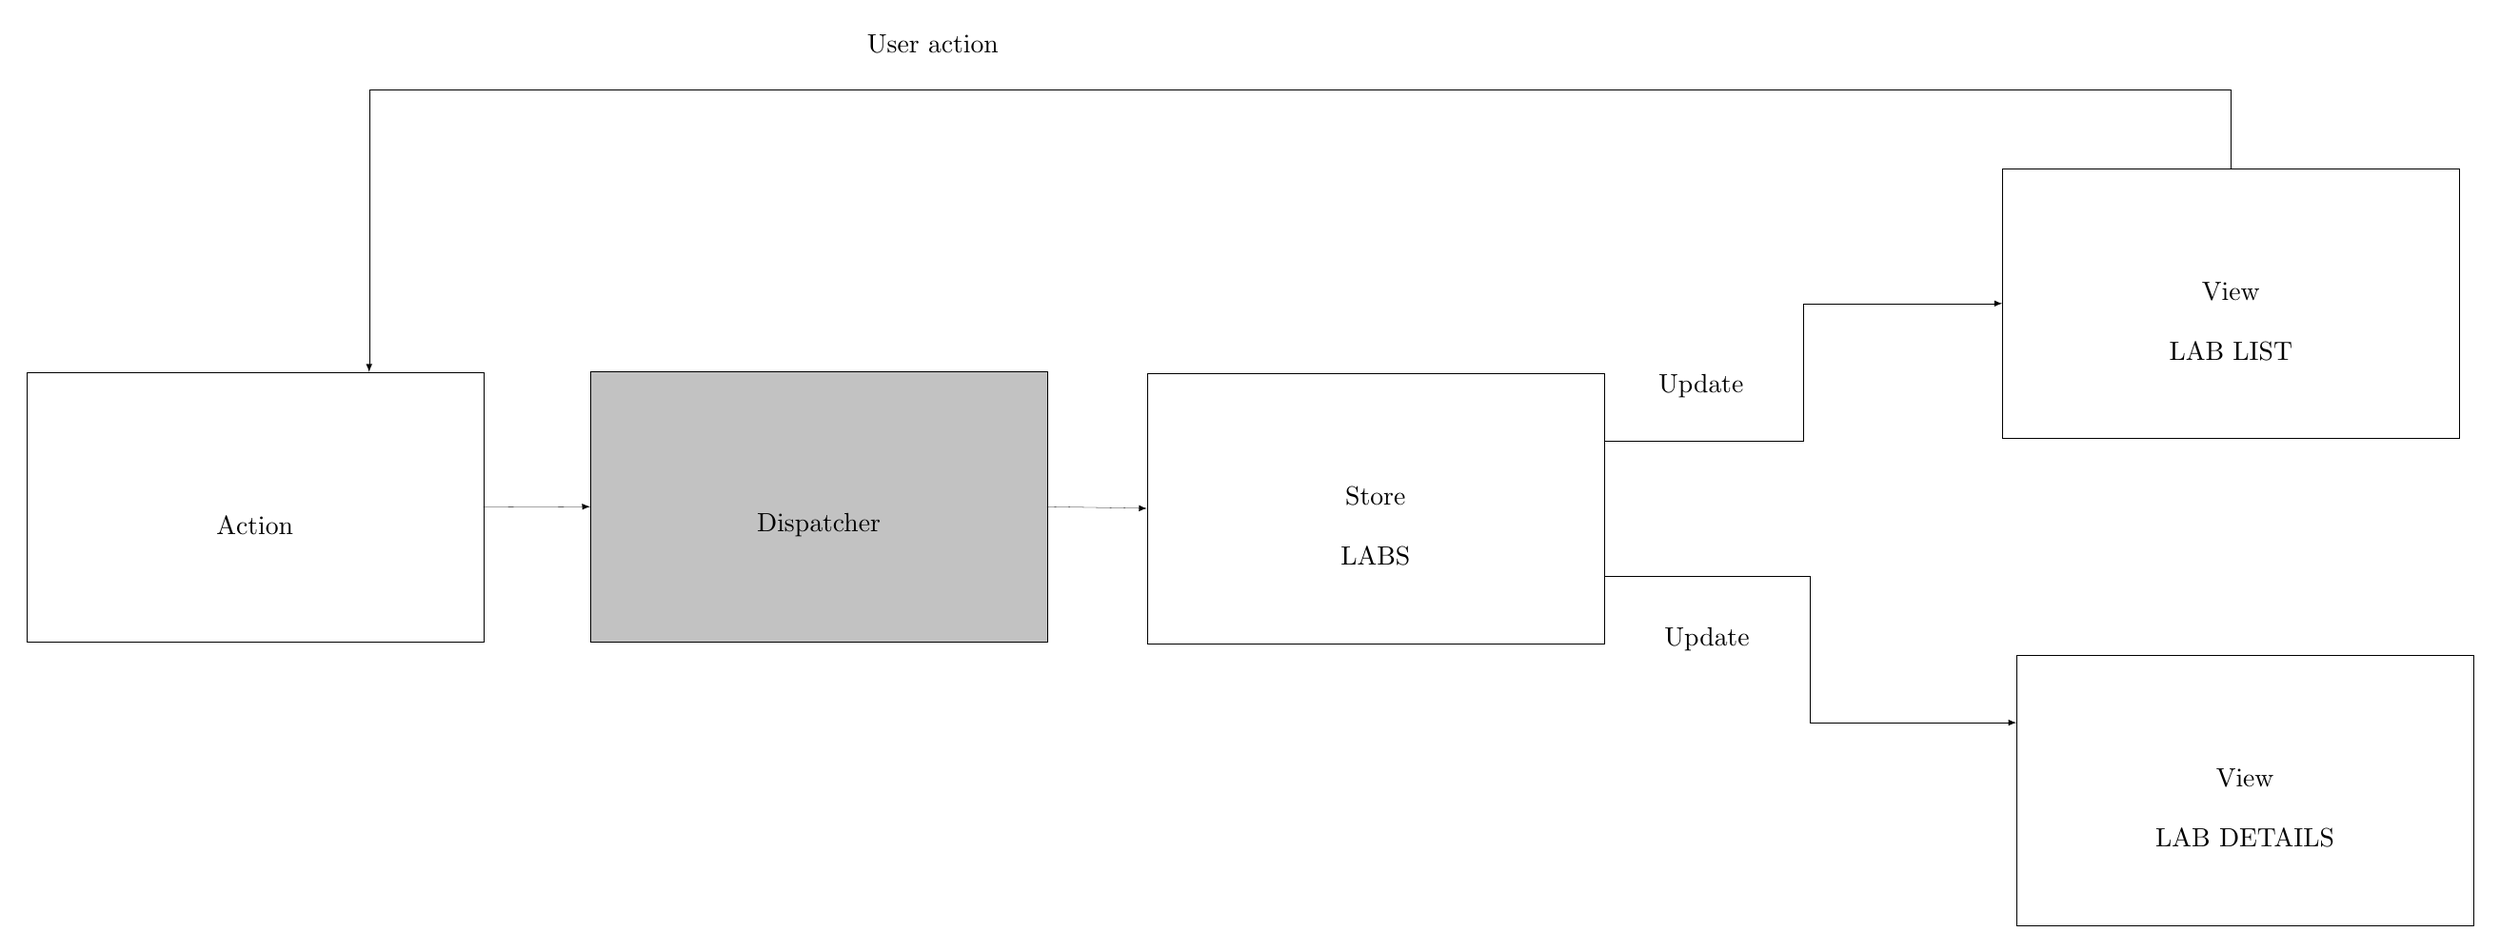
\begin{tikzpicture}
\pgftransformxscale{1.000000}
\pgftransformyscale{-1.000000}
\definecolor{dialinecolor}{rgb}{0.000000, 0.000000, 0.000000}
\pgfsetstrokecolor{dialinecolor}
\definecolor{dialinecolor}{rgb}{1.000000, 1.000000, 1.000000}
\pgfsetfillcolor{dialinecolor}
\definecolor{dialinecolor}{rgb}{1.000000, 1.000000, 1.000000}
\pgfsetfillcolor{dialinecolor}
\fill (30.127000\du,2.450020\du)--(30.127000\du,6.051412\du)--(36.221673\du,6.051412\du)--(36.221673\du,2.450020\du)--cycle;
\pgfsetlinewidth{0.100000\du}
\pgfsetdash{}{0pt}
\pgfsetdash{}{0pt}
\pgfsetmiterjoin
\definecolor{dialinecolor}{rgb}{0.000000, 0.000000, 0.000000}
\pgfsetstrokecolor{dialinecolor}
\draw (30.127000\du,2.450020\du)--(30.127000\du,6.051412\du)--(36.221673\du,6.051412\du)--(36.221673\du,2.450020\du)--cycle;
% setfont left to latex
\definecolor{dialinecolor}{rgb}{0.000000, 0.000000, 0.000000}
\pgfsetstrokecolor{dialinecolor}
\node at (33.174336\du,4.090716\du){View};
% setfont left to latex
\definecolor{dialinecolor}{rgb}{0.000000, 0.000000, 0.000000}
\pgfsetstrokecolor{dialinecolor}
\node at (33.174336\du,4.890716\du){LAB LIST};
\definecolor{dialinecolor}{rgb}{1.000000, 1.000000, 1.000000}
\pgfsetfillcolor{dialinecolor}
\fill (3.767030\du,5.167300\du)--(3.767030\du,8.768692\du)--(9.861703\du,8.768692\du)--(9.861703\du,5.167300\du)--cycle;
\pgfsetlinewidth{0.100000\du}
\pgfsetdash{}{0pt}
\pgfsetdash{}{0pt}
\pgfsetmiterjoin
\definecolor{dialinecolor}{rgb}{0.000000, 0.000000, 0.000000}
\pgfsetstrokecolor{dialinecolor}
\draw (3.767030\du,5.167300\du)--(3.767030\du,8.768692\du)--(9.861703\du,8.768692\du)--(9.861703\du,5.167300\du)--cycle;
% setfont left to latex
\definecolor{dialinecolor}{rgb}{0.000000, 0.000000, 0.000000}
\pgfsetstrokecolor{dialinecolor}
\node at (6.814366\du,7.207996\du){Action};
\definecolor{dialinecolor}{rgb}{0.760784, 0.760784, 0.760784}
\pgfsetfillcolor{dialinecolor}
\fill (11.288700\du,5.160520\du)--(11.288700\du,8.761912\du)--(17.383373\du,8.761912\du)--(17.383373\du,5.160520\du)--cycle;
\pgfsetlinewidth{0.100000\du}
\pgfsetdash{}{0pt}
\pgfsetdash{}{0pt}
\pgfsetmiterjoin
\definecolor{dialinecolor}{rgb}{0.000000, 0.000000, 0.000000}
\pgfsetstrokecolor{dialinecolor}
\draw (11.288700\du,5.160520\du)--(11.288700\du,8.761912\du)--(17.383373\du,8.761912\du)--(17.383373\du,5.160520\du)--cycle;
% setfont left to latex
\definecolor{dialinecolor}{rgb}{0.000000, 0.000000, 0.000000}
\pgfsetstrokecolor{dialinecolor}
\node at (14.336036\du,7.201216\du){Dispatcher};
\definecolor{dialinecolor}{rgb}{1.000000, 1.000000, 1.000000}
\pgfsetfillcolor{dialinecolor}
\fill (18.715500\du,5.183450\du)--(18.715500\du,8.784842\du)--(24.810173\du,8.784842\du)--(24.810173\du,5.183450\du)--cycle;
\pgfsetlinewidth{0.100000\du}
\pgfsetdash{}{0pt}
\pgfsetdash{}{0pt}
\pgfsetmiterjoin
\definecolor{dialinecolor}{rgb}{0.000000, 0.000000, 0.000000}
\pgfsetstrokecolor{dialinecolor}
\draw (18.715500\du,5.183450\du)--(18.715500\du,8.784842\du)--(24.810173\du,8.784842\du)--(24.810173\du,5.183450\du)--cycle;
% setfont left to latex
\definecolor{dialinecolor}{rgb}{0.000000, 0.000000, 0.000000}
\pgfsetstrokecolor{dialinecolor}
\node at (21.762836\du,6.824146\du){Store};
% setfont left to latex
\definecolor{dialinecolor}{rgb}{0.000000, 0.000000, 0.000000}
\pgfsetstrokecolor{dialinecolor}
\node at (21.762836\du,7.624146\du){LABS};
\definecolor{dialinecolor}{rgb}{1.000000, 1.000000, 1.000000}
\pgfsetfillcolor{dialinecolor}
\fill (30.314600\du,8.941950\du)--(30.314600\du,12.543342\du)--(36.409273\du,12.543342\du)--(36.409273\du,8.941950\du)--cycle;
\pgfsetlinewidth{0.100000\du}
\pgfsetdash{}{0pt}
\pgfsetdash{}{0pt}
\pgfsetmiterjoin
\definecolor{dialinecolor}{rgb}{0.000000, 0.000000, 0.000000}
\pgfsetstrokecolor{dialinecolor}
\draw (30.314600\du,8.941950\du)--(30.314600\du,12.543342\du)--(36.409273\du,12.543342\du)--(36.409273\du,8.941950\du)--cycle;
% setfont left to latex
\definecolor{dialinecolor}{rgb}{0.000000, 0.000000, 0.000000}
\pgfsetstrokecolor{dialinecolor}
\node at (33.361936\du,10.582646\du){View};
% setfont left to latex
\definecolor{dialinecolor}{rgb}{0.000000, 0.000000, 0.000000}
\pgfsetstrokecolor{dialinecolor}
\node at (33.361936\du,11.382646\du){LAB DETAILS};
\pgfsetlinewidth{0.100000\du}
\pgfsetdash{}{0pt}
\pgfsetdash{}{0pt}
\pgfsetbuttcap
{
\definecolor{dialinecolor}{rgb}{0.000000, 0.000000, 0.000000}
\pgfsetfillcolor{dialinecolor}
% was here!!!
\pgfsetarrowsend{latex}
\definecolor{dialinecolor}{rgb}{0.000000, 0.000000, 0.000000}
\pgfsetstrokecolor{dialinecolor}
\draw (9.861700\du,6.968000\du)--(11.288700\du,6.961216\du);
}
\pgfsetlinewidth{0.100000\du}
\pgfsetdash{}{0pt}
\pgfsetdash{}{0pt}
\pgfsetbuttcap
{
\definecolor{dialinecolor}{rgb}{0.000000, 0.000000, 0.000000}
\pgfsetfillcolor{dialinecolor}
% was here!!!
\pgfsetarrowsend{latex}
\definecolor{dialinecolor}{rgb}{0.000000, 0.000000, 0.000000}
\pgfsetstrokecolor{dialinecolor}
\draw (17.383373\du,6.961216\du)--(18.715500\du,6.984150\du);
}
\pgfsetlinewidth{0.100000\du}
\pgfsetdash{}{0pt}
\pgfsetdash{}{0pt}
\pgfsetmiterjoin
\pgfsetbuttcap
{
\definecolor{dialinecolor}{rgb}{0.000000, 0.000000, 0.000000}
\pgfsetfillcolor{dialinecolor}
% was here!!!
\pgfsetarrowsend{latex}
{\pgfsetcornersarced{\pgfpoint{0.000000\du}{0.000000\du}}\definecolor{dialinecolor}{rgb}{0.000000, 0.000000, 0.000000}
\pgfsetstrokecolor{dialinecolor}
\draw (24.810173\du,6.083798\du)--(27.468586\du,6.083798\du)--(27.468586\du,4.250716\du)--(30.127000\du,4.250716\du);
}}
\pgfsetlinewidth{0.100000\du}
\pgfsetdash{}{0pt}
\pgfsetdash{}{0pt}
\pgfsetmiterjoin
\pgfsetbuttcap
{
\definecolor{dialinecolor}{rgb}{0.000000, 0.000000, 0.000000}
\pgfsetfillcolor{dialinecolor}
% was here!!!
\pgfsetarrowsend{latex}
{\pgfsetcornersarced{\pgfpoint{0.000000\du}{0.000000\du}}\definecolor{dialinecolor}{rgb}{0.000000, 0.000000, 0.000000}
\pgfsetstrokecolor{dialinecolor}
\draw (24.810173\du,7.884494\du)--(27.562386\du,7.884494\du)--(27.562386\du,9.842298\du)--(30.314600\du,9.842298\du);
}}
\pgfsetlinewidth{0.100000\du}
\pgfsetdash{}{0pt}
\pgfsetdash{}{0pt}
\pgfsetmiterjoin
\pgfsetbuttcap
{
\definecolor{dialinecolor}{rgb}{0.000000, 0.000000, 0.000000}
\pgfsetfillcolor{dialinecolor}
% was here!!!
\pgfsetarrowsend{latex}
{\pgfsetcornersarced{\pgfpoint{0.000000\du}{0.000000\du}}\definecolor{dialinecolor}{rgb}{0.000000, 0.000000, 0.000000}
\pgfsetstrokecolor{dialinecolor}
\draw (33.174336\du,2.450020\du)--(33.174336\du,1.400020\du)--(8.338035\du,1.400020\du)--(8.338035\du,5.167300\du);
}}
% setfont left to latex
\definecolor{dialinecolor}{rgb}{0.000000, 0.000000, 0.000000}
\pgfsetstrokecolor{dialinecolor}
\node at (15.858400\du,0.790717\du){User action};
% setfont left to latex
\definecolor{dialinecolor}{rgb}{0.000000, 0.000000, 0.000000}
\pgfsetstrokecolor{dialinecolor}
\node at (26.105100\du,5.356830\du){Update};
% setfont left to latex
\definecolor{dialinecolor}{rgb}{0.000000, 0.000000, 0.000000}
\pgfsetstrokecolor{dialinecolor}
\node at (26.184500\du,8.726810\du){Update};
\end{tikzpicture}
}}
\caption{The Flux architecture.}
\end{figure}


\todo{Change the figure above to a more general Flux figure}


\subsection{Why not use MVC?}

Model-view-controller, or MVC, is the most used architecture for the web today. The architecture is devided into three main roles;
\begin{itemize}  
\item \emph{Model:} Holds all the data
\item \emph{View:} Represents the model (data) in the user interface
\item \emph{Controller:} Handles manipulation of the data and moves it around.\ldots 
\end{itemize}

Writing JavaScript with an MVC pattern works well, however, logic or updating the user interface can be very complex. The team behind React chose to use Flux as the main architectual pattern, since the data flow in the application can be managed fairly easy. Simple components can be implemented using an MVC approach, but as we experienced, it gets tricky when the scale of the application grows. As seen in the figure below \worry{Place figure below!!!}, the main problem with React in MVC is having multiple views that communicate bidirectional.

\begin{figure}[h]
\centering
\scalebox{1}{{% Graphic for TeX using PGF
% Title: /home/tomgli/workspace/github.com/bachopp/thesis/files/chapters/background/graphs/MVC_dilemma.dia
% Creator: Dia v0.97.3
% CreationDate: Sat May 14 15:09:59 2016
% For: tomgli
% \usepackage{tikz}
% The following commands are not supported in PSTricks at present
% We define them conditionally, so when they are implemented,
% this pgf file will use them.
\ifx\du\undefined
  \newlength{\du}
\fi
\setlength{\du}{15\unitlength}
\begin{tikzpicture}
\pgftransformxscale{1.000000}
\pgftransformyscale{-1.000000}
\definecolor{dialinecolor}{rgb}{0.000000, 0.000000, 0.000000}
\pgfsetstrokecolor{dialinecolor}
\definecolor{dialinecolor}{rgb}{1.000000, 1.000000, 1.000000}
\pgfsetfillcolor{dialinecolor}
\definecolor{dialinecolor}{rgb}{1.000000, 1.000000, 1.000000}
\pgfsetfillcolor{dialinecolor}
\fill (15.491700\du,8.673930\du)--(15.491700\du,11.573930\du)--(19.664590\du,11.573930\du)--(19.664590\du,8.673930\du)--cycle;
\pgfsetlinewidth{0.100000\du}
\pgfsetdash{}{0pt}
\pgfsetdash{}{0pt}
\pgfsetmiterjoin
\definecolor{dialinecolor}{rgb}{0.000000, 0.000000, 0.000000}
\pgfsetstrokecolor{dialinecolor}
\draw (15.491700\du,8.673930\du)--(15.491700\du,11.573930\du)--(19.664590\du,11.573930\du)--(19.664590\du,8.673930\du)--cycle;
% setfont left to latex
\definecolor{dialinecolor}{rgb}{0.000000, 0.000000, 0.000000}
\pgfsetstrokecolor{dialinecolor}
\node at (17.578145\du,10.323930\du){Action};
\definecolor{dialinecolor}{rgb}{1.000000, 1.000000, 1.000000}
\pgfsetfillcolor{dialinecolor}
\fill (21.174600\du,8.688020\du)--(21.174600\du,11.588020\du)--(28.569600\du,11.588020\du)--(28.569600\du,8.688020\du)--cycle;
\pgfsetlinewidth{0.100000\du}
\pgfsetdash{}{0pt}
\pgfsetdash{}{0pt}
\pgfsetmiterjoin
\definecolor{dialinecolor}{rgb}{0.000000, 0.000000, 0.000000}
\pgfsetstrokecolor{dialinecolor}
\draw (21.174600\du,8.688020\du)--(21.174600\du,11.588020\du)--(28.569600\du,11.588020\du)--(28.569600\du,8.688020\du)--cycle;
% setfont left to latex
\definecolor{dialinecolor}{rgb}{0.000000, 0.000000, 0.000000}
\pgfsetstrokecolor{dialinecolor}
\node at (24.872100\du,10.338020\du){Controller};
\pgfsetlinewidth{0.100000\du}
\pgfsetdash{}{0pt}
\pgfsetdash{}{0pt}
\pgfsetbuttcap
{
\definecolor{dialinecolor}{rgb}{0.000000, 0.000000, 0.000000}
\pgfsetfillcolor{dialinecolor}
% was here!!!
\pgfsetarrowsend{stealth}
\definecolor{dialinecolor}{rgb}{0.000000, 0.000000, 0.000000}
\pgfsetstrokecolor{dialinecolor}
\draw (19.664590\du,10.123930\du)--(21.174600\du,10.138020\du);
}
\pgfsetlinewidth{0.100000\du}
\pgfsetdash{}{0pt}
\pgfsetdash{}{0pt}
\pgfsetbuttcap
{
\definecolor{dialinecolor}{rgb}{0.000000, 0.000000, 0.000000}
\pgfsetfillcolor{dialinecolor}
% was here!!!
\pgfsetarrowsend{stealth}
\definecolor{dialinecolor}{rgb}{0.000000, 0.000000, 0.000000}
\pgfsetstrokecolor{dialinecolor}
\draw (28.569600\du,10.138020\du)--(31.316900\du,5.509640\du);
}
\definecolor{dialinecolor}{rgb}{1.000000, 1.000000, 1.000000}
\pgfsetfillcolor{dialinecolor}
\fill (31.316900\du,4.559640\du)--(31.316900\du,6.459640\du)--(34.880193\du,6.459640\du)--(34.880193\du,4.559640\du)--cycle;
\pgfsetlinewidth{0.100000\du}
\pgfsetdash{}{0pt}
\pgfsetdash{}{0pt}
\pgfsetmiterjoin
\definecolor{dialinecolor}{rgb}{0.000000, 0.000000, 0.000000}
\pgfsetstrokecolor{dialinecolor}
\draw (31.316900\du,4.559640\du)--(31.316900\du,6.459640\du)--(34.880193\du,6.459640\du)--(34.880193\du,4.559640\du)--cycle;
% setfont left to latex
\definecolor{dialinecolor}{rgb}{0.000000, 0.000000, 0.000000}
\pgfsetstrokecolor{dialinecolor}
\node at (33.098546\du,5.704640\du){Model};
\definecolor{dialinecolor}{rgb}{1.000000, 1.000000, 1.000000}
\pgfsetfillcolor{dialinecolor}
\fill (31.614200\du,6.194790\du)--(31.614200\du,8.094790\du)--(35.177493\du,8.094790\du)--(35.177493\du,6.194790\du)--cycle;
\pgfsetlinewidth{0.100000\du}
\pgfsetdash{}{0pt}
\pgfsetdash{}{0pt}
\pgfsetmiterjoin
\definecolor{dialinecolor}{rgb}{0.000000, 0.000000, 0.000000}
\pgfsetstrokecolor{dialinecolor}
\draw (31.614200\du,6.194790\du)--(31.614200\du,8.094790\du)--(35.177493\du,8.094790\du)--(35.177493\du,6.194790\du)--cycle;
% setfont left to latex
\definecolor{dialinecolor}{rgb}{0.000000, 0.000000, 0.000000}
\pgfsetstrokecolor{dialinecolor}
\node at (33.395846\du,7.339790\du){Model};
\definecolor{dialinecolor}{rgb}{1.000000, 1.000000, 1.000000}
\pgfsetfillcolor{dialinecolor}
\fill (31.346600\du,13.627200\du)--(31.346600\du,15.527200\du)--(34.909893\du,15.527200\du)--(34.909893\du,13.627200\du)--cycle;
\pgfsetlinewidth{0.100000\du}
\pgfsetdash{}{0pt}
\pgfsetdash{}{0pt}
\pgfsetmiterjoin
\definecolor{dialinecolor}{rgb}{0.000000, 0.000000, 0.000000}
\pgfsetstrokecolor{dialinecolor}
\draw (31.346600\du,13.627200\du)--(31.346600\du,15.527200\du)--(34.909893\du,15.527200\du)--(34.909893\du,13.627200\du)--cycle;
% setfont left to latex
\definecolor{dialinecolor}{rgb}{0.000000, 0.000000, 0.000000}
\pgfsetstrokecolor{dialinecolor}
\node at (33.128246\du,14.772200\du){Model};
\definecolor{dialinecolor}{rgb}{1.000000, 1.000000, 1.000000}
\pgfsetfillcolor{dialinecolor}
\fill (31.643900\du,11.992100\du)--(31.643900\du,13.892100\du)--(35.207193\du,13.892100\du)--(35.207193\du,11.992100\du)--cycle;
\pgfsetlinewidth{0.100000\du}
\pgfsetdash{}{0pt}
\pgfsetdash{}{0pt}
\pgfsetmiterjoin
\definecolor{dialinecolor}{rgb}{0.000000, 0.000000, 0.000000}
\pgfsetstrokecolor{dialinecolor}
\draw (31.643900\du,11.992100\du)--(31.643900\du,13.892100\du)--(35.207193\du,13.892100\du)--(35.207193\du,11.992100\du)--cycle;
% setfont left to latex
\definecolor{dialinecolor}{rgb}{0.000000, 0.000000, 0.000000}
\pgfsetstrokecolor{dialinecolor}
\node at (33.425546\du,13.137100\du){Model};
\definecolor{dialinecolor}{rgb}{1.000000, 1.000000, 1.000000}
\pgfsetfillcolor{dialinecolor}
\fill (31.941200\du,10.357000\du)--(31.941200\du,12.257000\du)--(35.504493\du,12.257000\du)--(35.504493\du,10.357000\du)--cycle;
\pgfsetlinewidth{0.100000\du}
\pgfsetdash{}{0pt}
\pgfsetdash{}{0pt}
\pgfsetmiterjoin
\definecolor{dialinecolor}{rgb}{0.000000, 0.000000, 0.000000}
\pgfsetstrokecolor{dialinecolor}
\draw (31.941200\du,10.357000\du)--(31.941200\du,12.257000\du)--(35.504493\du,12.257000\du)--(35.504493\du,10.357000\du)--cycle;
% setfont left to latex
\definecolor{dialinecolor}{rgb}{0.000000, 0.000000, 0.000000}
\pgfsetstrokecolor{dialinecolor}
\node at (33.722846\du,11.502000\du){Model};
\definecolor{dialinecolor}{rgb}{1.000000, 1.000000, 1.000000}
\pgfsetfillcolor{dialinecolor}
\fill (37.726500\du,4.447150\du)--(37.726500\du,6.347150\du)--(41.289793\du,6.347150\du)--(41.289793\du,4.447150\du)--cycle;
\pgfsetlinewidth{0.100000\du}
\pgfsetdash{}{0pt}
\pgfsetdash{}{0pt}
\pgfsetmiterjoin
\definecolor{dialinecolor}{rgb}{0.000000, 0.000000, 0.000000}
\pgfsetstrokecolor{dialinecolor}
\draw (37.726500\du,4.447150\du)--(37.726500\du,6.347150\du)--(41.289793\du,6.347150\du)--(41.289793\du,4.447150\du)--cycle;
% setfont left to latex
\definecolor{dialinecolor}{rgb}{0.000000, 0.000000, 0.000000}
\pgfsetstrokecolor{dialinecolor}
\node at (39.508146\du,5.592150\du){View};
\definecolor{dialinecolor}{rgb}{1.000000, 1.000000, 1.000000}
\pgfsetfillcolor{dialinecolor}
\fill (38.006100\du,6.135330\du)--(38.006100\du,8.035330\du)--(41.569393\du,8.035330\du)--(41.569393\du,6.135330\du)--cycle;
\pgfsetlinewidth{0.100000\du}
\pgfsetdash{}{0pt}
\pgfsetdash{}{0pt}
\pgfsetmiterjoin
\definecolor{dialinecolor}{rgb}{0.000000, 0.000000, 0.000000}
\pgfsetstrokecolor{dialinecolor}
\draw (38.006100\du,6.135330\du)--(38.006100\du,8.035330\du)--(41.569393\du,8.035330\du)--(41.569393\du,6.135330\du)--cycle;
% setfont left to latex
\definecolor{dialinecolor}{rgb}{0.000000, 0.000000, 0.000000}
\pgfsetstrokecolor{dialinecolor}
\node at (39.787746\du,7.280330\du){View};
\definecolor{dialinecolor}{rgb}{1.000000, 1.000000, 1.000000}
\pgfsetfillcolor{dialinecolor}
\fill (38.303400\du,7.770470\du)--(38.303400\du,9.670470\du)--(41.866693\du,9.670470\du)--(41.866693\du,7.770470\du)--cycle;
\pgfsetlinewidth{0.100000\du}
\pgfsetdash{}{0pt}
\pgfsetdash{}{0pt}
\pgfsetmiterjoin
\definecolor{dialinecolor}{rgb}{0.000000, 0.000000, 0.000000}
\pgfsetstrokecolor{dialinecolor}
\draw (38.303400\du,7.770470\du)--(38.303400\du,9.670470\du)--(41.866693\du,9.670470\du)--(41.866693\du,7.770470\du)--cycle;
% setfont left to latex
\definecolor{dialinecolor}{rgb}{0.000000, 0.000000, 0.000000}
\pgfsetstrokecolor{dialinecolor}
\node at (40.085046\du,8.915470\du){View};
\definecolor{dialinecolor}{rgb}{1.000000, 1.000000, 1.000000}
\pgfsetfillcolor{dialinecolor}
\fill (37.738600\du,13.567800\du)--(37.738600\du,15.467800\du)--(41.301893\du,15.467800\du)--(41.301893\du,13.567800\du)--cycle;
\pgfsetlinewidth{0.100000\du}
\pgfsetdash{}{0pt}
\pgfsetdash{}{0pt}
\pgfsetmiterjoin
\definecolor{dialinecolor}{rgb}{0.000000, 0.000000, 0.000000}
\pgfsetstrokecolor{dialinecolor}
\draw (37.738600\du,13.567800\du)--(37.738600\du,15.467800\du)--(41.301893\du,15.467800\du)--(41.301893\du,13.567800\du)--cycle;
% setfont left to latex
\definecolor{dialinecolor}{rgb}{0.000000, 0.000000, 0.000000}
\pgfsetstrokecolor{dialinecolor}
\node at (39.520246\du,14.712800\du){View};
\definecolor{dialinecolor}{rgb}{1.000000, 1.000000, 1.000000}
\pgfsetfillcolor{dialinecolor}
\fill (38.035900\du,11.932600\du)--(38.035900\du,13.832600\du)--(41.599193\du,13.832600\du)--(41.599193\du,11.932600\du)--cycle;
\pgfsetlinewidth{0.100000\du}
\pgfsetdash{}{0pt}
\pgfsetdash{}{0pt}
\pgfsetmiterjoin
\definecolor{dialinecolor}{rgb}{0.000000, 0.000000, 0.000000}
\pgfsetstrokecolor{dialinecolor}
\draw (38.035900\du,11.932600\du)--(38.035900\du,13.832600\du)--(41.599193\du,13.832600\du)--(41.599193\du,11.932600\du)--cycle;
% setfont left to latex
\definecolor{dialinecolor}{rgb}{0.000000, 0.000000, 0.000000}
\pgfsetstrokecolor{dialinecolor}
\node at (39.817546\du,13.077600\du){View};
\definecolor{dialinecolor}{rgb}{1.000000, 1.000000, 1.000000}
\pgfsetfillcolor{dialinecolor}
\fill (38.333200\du,10.297500\du)--(38.333200\du,12.197500\du)--(41.896493\du,12.197500\du)--(41.896493\du,10.297500\du)--cycle;
\pgfsetlinewidth{0.100000\du}
\pgfsetdash{}{0pt}
\pgfsetdash{}{0pt}
\pgfsetmiterjoin
\definecolor{dialinecolor}{rgb}{0.000000, 0.000000, 0.000000}
\pgfsetstrokecolor{dialinecolor}
\draw (38.333200\du,10.297500\du)--(38.333200\du,12.197500\du)--(41.896493\du,12.197500\du)--(41.896493\du,10.297500\du)--cycle;
% setfont left to latex
\definecolor{dialinecolor}{rgb}{0.000000, 0.000000, 0.000000}
\pgfsetstrokecolor{dialinecolor}
\node at (40.114846\du,11.442500\du){View};
\pgfsetlinewidth{0.100000\du}
\pgfsetdash{}{0pt}
\pgfsetdash{}{0pt}
\pgfsetbuttcap
{
\definecolor{dialinecolor}{rgb}{0.000000, 0.000000, 0.000000}
\pgfsetfillcolor{dialinecolor}
% was here!!!
\pgfsetarrowsend{stealth}
\definecolor{dialinecolor}{rgb}{0.000000, 0.000000, 0.000000}
\pgfsetstrokecolor{dialinecolor}
\draw (28.569600\du,10.138020\du)--(31.614200\du,7.144790\du);
}
\pgfsetlinewidth{0.100000\du}
\pgfsetdash{}{0pt}
\pgfsetdash{}{0pt}
\pgfsetbuttcap
{
\definecolor{dialinecolor}{rgb}{0.000000, 0.000000, 0.000000}
\pgfsetfillcolor{dialinecolor}
% was here!!!
\pgfsetarrowsend{stealth}
\definecolor{dialinecolor}{rgb}{0.000000, 0.000000, 0.000000}
\pgfsetstrokecolor{dialinecolor}
\draw (28.569600\du,10.138020\du)--(31.962800\du,8.729000\du);
}
\pgfsetlinewidth{0.100000\du}
\pgfsetdash{}{0pt}
\pgfsetdash{}{0pt}
\pgfsetbuttcap
{
\definecolor{dialinecolor}{rgb}{0.000000, 0.000000, 0.000000}
\pgfsetfillcolor{dialinecolor}
% was here!!!
\pgfsetarrowsend{stealth}
\definecolor{dialinecolor}{rgb}{0.000000, 0.000000, 0.000000}
\pgfsetstrokecolor{dialinecolor}
\draw (28.569600\du,10.138020\du)--(31.941200\du,11.307000\du);
}
\pgfsetlinewidth{0.100000\du}
\pgfsetdash{}{0pt}
\pgfsetdash{}{0pt}
\pgfsetbuttcap
{
\definecolor{dialinecolor}{rgb}{0.000000, 0.000000, 0.000000}
\pgfsetfillcolor{dialinecolor}
% was here!!!
\pgfsetarrowsend{stealth}
\definecolor{dialinecolor}{rgb}{0.000000, 0.000000, 0.000000}
\pgfsetstrokecolor{dialinecolor}
\draw (28.569600\du,10.138020\du)--(31.573200\du,12.894500\du);
}
\pgfsetlinewidth{0.100000\du}
\pgfsetdash{}{0pt}
\pgfsetdash{}{0pt}
\pgfsetbuttcap
{
\definecolor{dialinecolor}{rgb}{0.000000, 0.000000, 0.000000}
\pgfsetfillcolor{dialinecolor}
% was here!!!
\pgfsetarrowsend{stealth}
\definecolor{dialinecolor}{rgb}{0.000000, 0.000000, 0.000000}
\pgfsetstrokecolor{dialinecolor}
\draw (28.569600\du,10.138020\du)--(31.346600\du,14.577200\du);
}
\pgfsetlinewidth{0.100000\du}
\pgfsetdash{}{0pt}
\pgfsetdash{}{0pt}
\pgfsetbuttcap
{
\definecolor{dialinecolor}{rgb}{0.000000, 0.000000, 0.000000}
\pgfsetfillcolor{dialinecolor}
% was here!!!
\pgfsetarrowsend{stealth}
\definecolor{dialinecolor}{rgb}{0.000000, 0.000000, 0.000000}
\pgfsetstrokecolor{dialinecolor}
\draw (34.909900\du,14.577200\du)--(37.738600\du,14.517800\du);
}
\pgfsetlinewidth{0.100000\du}
\pgfsetdash{}{0pt}
\pgfsetdash{}{0pt}
\pgfsetbuttcap
{
\definecolor{dialinecolor}{rgb}{0.000000, 0.000000, 0.000000}
\pgfsetfillcolor{dialinecolor}
% was here!!!
\pgfsetarrowsend{stealth}
\definecolor{dialinecolor}{rgb}{0.000000, 0.000000, 0.000000}
\pgfsetstrokecolor{dialinecolor}
\draw (35.207200\du,12.942100\du)--(38.035900\du,12.882600\du);
}
\pgfsetlinewidth{0.100000\du}
\pgfsetdash{}{0pt}
\pgfsetdash{}{0pt}
\pgfsetbuttcap
{
\definecolor{dialinecolor}{rgb}{0.000000, 0.000000, 0.000000}
\pgfsetfillcolor{dialinecolor}
% was here!!!
\pgfsetarrowsend{stealth}
\definecolor{dialinecolor}{rgb}{0.000000, 0.000000, 0.000000}
\pgfsetstrokecolor{dialinecolor}
\draw (35.504500\du,11.307000\du)--(38.333200\du,11.247500\du);
}
\definecolor{dialinecolor}{rgb}{1.000000, 1.000000, 1.000000}
\pgfsetfillcolor{dialinecolor}
\fill (31.962800\du,7.779000\du)--(31.962800\du,9.679000\du)--(35.526093\du,9.679000\du)--(35.526093\du,7.779000\du)--cycle;
\pgfsetlinewidth{0.100000\du}
\pgfsetdash{}{0pt}
\pgfsetdash{}{0pt}
\pgfsetmiterjoin
\definecolor{dialinecolor}{rgb}{0.000000, 0.000000, 0.000000}
\pgfsetstrokecolor{dialinecolor}
\draw (31.962800\du,7.779000\du)--(31.962800\du,9.679000\du)--(35.526093\du,9.679000\du)--(35.526093\du,7.779000\du)--cycle;
% setfont left to latex
\definecolor{dialinecolor}{rgb}{0.000000, 0.000000, 0.000000}
\pgfsetstrokecolor{dialinecolor}
\node at (33.744446\du,8.924000\du){Model};
\pgfsetlinewidth{0.100000\du}
\pgfsetdash{}{0pt}
\pgfsetdash{}{0pt}
\pgfsetbuttcap
{
\definecolor{dialinecolor}{rgb}{0.000000, 0.000000, 0.000000}
\pgfsetfillcolor{dialinecolor}
% was here!!!
\pgfsetarrowsend{stealth}
\definecolor{dialinecolor}{rgb}{0.000000, 0.000000, 0.000000}
\pgfsetstrokecolor{dialinecolor}
\draw (35.526100\du,8.729000\du)--(38.303400\du,8.720470\du);
}
\pgfsetlinewidth{0.100000\du}
\pgfsetdash{}{0pt}
\pgfsetdash{}{0pt}
\pgfsetbuttcap
{
\definecolor{dialinecolor}{rgb}{0.000000, 0.000000, 0.000000}
\pgfsetfillcolor{dialinecolor}
% was here!!!
\pgfsetarrowsend{stealth}
\definecolor{dialinecolor}{rgb}{0.000000, 0.000000, 0.000000}
\pgfsetstrokecolor{dialinecolor}
\draw (35.239200\du,7.109770\du)--(38.006100\du,7.085330\du);
}
\pgfsetlinewidth{0.100000\du}
\pgfsetdash{}{0pt}
\pgfsetdash{}{0pt}
\pgfsetbuttcap
{
\definecolor{dialinecolor}{rgb}{0.000000, 0.000000, 0.000000}
\pgfsetfillcolor{dialinecolor}
% was here!!!
\pgfsetarrowsend{stealth}
\definecolor{dialinecolor}{rgb}{0.000000, 0.000000, 0.000000}
\pgfsetstrokecolor{dialinecolor}
\draw (34.880200\du,5.509640\du)--(37.726500\du,5.397150\du);
}
\pgfsetlinewidth{0.100000\du}
\pgfsetdash{}{0pt}
\pgfsetdash{}{0pt}
\pgfsetbuttcap
{
\definecolor{dialinecolor}{rgb}{0.000000, 0.000000, 0.000000}
\pgfsetfillcolor{dialinecolor}
% was here!!!
\pgfsetarrowsend{stealth}
\definecolor{dialinecolor}{rgb}{0.000000, 0.000000, 0.000000}
\pgfsetstrokecolor{dialinecolor}
\draw (35.504500\du,11.307000\du)--(37.738600\du,13.567800\du);
}
\pgfsetlinewidth{0.100000\du}
\pgfsetdash{}{0pt}
\pgfsetdash{}{0pt}
\pgfsetbuttcap
{
\definecolor{dialinecolor}{rgb}{0.000000, 0.000000, 0.000000}
\pgfsetfillcolor{dialinecolor}
% was here!!!
\pgfsetarrowsend{stealth}
\definecolor{dialinecolor}{rgb}{0.000000, 0.000000, 0.000000}
\pgfsetstrokecolor{dialinecolor}
\draw (35.526100\du,8.729000\du)--(37.726500\du,6.347150\du);
}
\pgfsetlinewidth{0.100000\du}
\pgfsetdash{}{0pt}
\pgfsetdash{}{0pt}
\pgfsetbuttcap
{
\definecolor{dialinecolor}{rgb}{0.000000, 0.000000, 0.000000}
\pgfsetfillcolor{dialinecolor}
% was here!!!
\pgfsetarrowsend{stealth}
\definecolor{dialinecolor}{rgb}{0.000000, 0.000000, 0.000000}
\pgfsetstrokecolor{dialinecolor}
\draw (38.333200\du,10.297500\du)--(35.526100\du,9.679000\du);
}
\pgfsetlinewidth{0.100000\du}
\pgfsetdash{}{0pt}
\pgfsetdash{}{0pt}
\pgfsetbuttcap
{
\definecolor{dialinecolor}{rgb}{0.000000, 0.000000, 0.000000}
\pgfsetfillcolor{dialinecolor}
% was here!!!
\pgfsetarrowsend{stealth}
\definecolor{dialinecolor}{rgb}{0.000000, 0.000000, 0.000000}
\pgfsetstrokecolor{dialinecolor}
\draw (38.303400\du,8.720470\du)--(35.504500\du,10.357000\du);
}
\end{tikzpicture}
}}
\caption{The biggest dilemma with MVC is scalability.}
\end{figure}

The data flow in MVC is bidirectional, meaning that the data will be sent to and from the view. As said, the data is directly connected to the view, and changes will trigger updates on both sides. Problems can emerge if the triggers cascading effects to the data, without having control of where the data is changed. Data can easily come out of hand, and parts of the application can be outdated. Changes in the data can be hard to trace, and debugging can be hard. As seen in the figure above \worry{ref til figure above} handling changes in data can be hard. Since the communication goes both ways, some parts of the system may have problems updating when the system grows.

